\documentclass[border=3pt,tikz]{standalone}
\usepackage{amsmath,amssymb}
\usepackage{bm} % math bold
\usepackage{tikz}
\usetikzlibrary{patterns}
\tikzset{>=latex}

\colorlet{myblue}{black!50!blue}
\colorlet{myred}{black!50!red}

\begin{document}


% RESISTANCE vs. TEMPERATURE
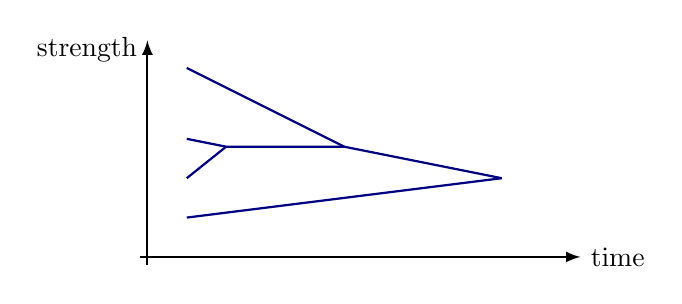
\begin{tikzpicture}
  \def\N{20}
  \def\xmin{-0.1} \def\xmax{5.0}
  \def\ymin{-0.1} \def\ymax{2.5}
  
  \coordinate (EM)  at (0.5,1.5);
  \coordinate (W)   at (0.5,1.0);
  \coordinate (S)   at (0.5,2.4);
  \coordinate (G)   at (0.5,0.5);
  
  \coordinate (EW)  at (1.0,1.4);
  \coordinate (GUT) at (2.5,1.4);
  \coordinate (P)   at (4.5,1.0);
  
  \draw[->,thick]
    (\xmin,0) -- (1.1*\xmax,0) node[right] {time};
  \draw[->,thick]
    (0,\ymin) -- (0,1.1*\ymax) node[above=5pt,below left,align=center] {strength};  

  \draw[thick,myblue]
     (EM) -- (EW) -- (GUT) -- (P);
     
  \draw[thick,myblue]
     (W) -- (EW);
     
  \draw[thick,myblue]
     (S) -- (GUT);
     
  \draw[thick,myblue]
     (G) -- (P);
  
\end{tikzpicture}



\end{document}
